\documentclass{article}
\usepackage{amsfonts, amsmath, amssymb, amsthm} % Math notations imported
\usepackage{enumitem}
\usepackage[margin=1in]{geometry}
\usepackage{graphicx}
\graphicspath{{./images/}}

\newtheorem{thm}{Theorem}
\newtheorem{prop}[thm]{Proposition}
\newtheorem{cor}[thm]{Corollary}

% title information
\title{Math 170A HW2}
\author{Neo Lee}
\date{04/14/2023}

% main content
\begin{document} 

% placing title information; comment out if using fancyhdr
\maketitle 

\textbf{Problem 1.}
\begin{enumerate}[label={\alph*)}]
    \item 
    Let $U\vec{x}=\vec{b}$ be
    \begin{align}
        \begin{bmatrix}
            u_{1,1} & u_{1,2} & \cdots & u_{1,n} \\
            0 & u_{2,2} & \cdots & u_{2,n} \\
            \vdots & \vdots & \ddots & \vdots \\
            0 & 0 & 0 & u_{n,n}
        \end{bmatrix}
        \begin{bmatrix}
            x_1 \\
            x_2 \\
            \vdots \\
            x_n
        \end{bmatrix}
        = 
        \begin{bmatrix}
            b_1 \\
            b_2 \\
            \vdots \\
            b_n
        \end{bmatrix}
        \nonumber
    \end{align}

    Then, we can perform backward substitution, starting from solving $x_n$ with row $n$.
    The exact formula would be $x_i = \frac{1}{u_{i,i}}\left(b_i - \sum\limits_{k=i+1}^nx_k\cdot u_{i,k}\right)$ for $i \in [1,n]$.

    \item \qquad
    \begin{figure}[h]
        \centering
        \includegraphics*[scale=0.5]{solve_upper_tri.png}
    \end{figure}

    \item
    For $i \in [1,n]$, there are $n-i$ multiplications, $n-i$ subtractions, and 1 division.
    Therefore, there are a total of $\sum\limits_{i=1}^n[2(n-i) + 1] = 2n^2 + n -2\sum\limits_{i=1}^{n}i=2n^2+n-2\times\frac{(1+n)n}{2} = 2n^2+n-n-n^2=n^2$ flops.
\end{enumerate}
\bigbreak

\textbf{Problem 2.}
\begin{enumerate}[label={\alph*)}]
    \item 
    Let $LA = U$, $c$ be some constant, and 
    \begin{align}
        L = 
        \begin{bmatrix}
            1 & c & \cdots & c \\
            m_{2,1} & 1 & \cdots & c \\
            \vdots & \vdots & \ddots & \vdots \\
            m_{n,1} & m_{n,2} & \cdots & 1
        \end{bmatrix}. \nonumber
    \end{align}
    Then, for each row $i \in [1,n]$ and column $k\in [i,n]$ in $U$, $u_{i, k} = a_{i, k} + \sum\limits_{j\in[1,i-1]}m_{i, j}\times a_{j,k} + C$, in which $a_{i,k}$ is basically the row $i$ and the summation term is basically the elementary transformation of summing all $j$ rows times the multipliers $m$.

    \item

\end{enumerate}
\bigbreak

\textbf{Problem 3.}
\begin{enumerate}[label={\alph*)}]
    \item 
    Let $L_1 \cdot L_2 = L_3$.
    Then, $l_3^{(i, j)} = \sum\limits_{k=1}^{n}l_1^{(i,k)}\times l_2^{(k,j)}$. Note that for $i < k$, $l_1^{(i,k)} = 0$ and for $k < j$, $l_2^{(k,j)} = 0$.
    Then, when $i < j$, for all $k\in [1,n]$, $i<k$ or $k<j$ must be true $\Rightarrow l_1^{(i,k)}\times l_2^{(k,j)}=0 \Rightarrow l_3^{i,j} = 0 \Rightarrow$  all the entries above diagonal are 0 $\Rightarrow L_3$ is lower triangular.

    \item 
    Let arbitrary lower triangular matrix $L_1, L_2, L_3$. $L_1 \cdot L_2 = L_3 \Leftrightarrow (L_1\cdot L_2)^T = L_3^T \Leftrightarrow L_2^T \cdot L_1^T = L_3^T \Leftrightarrow U_2 \cdot U_1 = U_3$.
    Hence, we get any arbitrary upper triangular matrix multiplication would get an upper triangular matrix.
\end{enumerate}
\bigbreak

\textbf{Problem 4.}
\begin{prop}
    LU factorization is unique.
\end{prop}
\begin{proof}
    Assume to the contrary that there exists $LU = \tilde{L}\tilde{U}$ such that $L \neq \tilde{L}$ and $U \neq \tilde{U}$.
    Then, $LU = \tilde{L}\tilde{U} \Leftrightarrow L = \tilde{L}\tilde{U}U^{-1} \Leftrightarrow \tilde{L}^{-1}L = \tilde{U}U^{-1}$.
    Since inverse of a lower triangular matrix is a lower triangular matrix, and the same holds for upper triangular matrix, we can see that the left hand side of the equation is a lower triangular matrix while the right hand side is an upper triangular matrix, which is impossible.
    Hence, contradiction is reached, and the proposition is proved.
\end{proof}
\bigbreak

\textbf{Problem 5.}
\begin{figure}[htb]
    \qquad
    \begin{minipage}{.4\textwidth}
        \centering
        {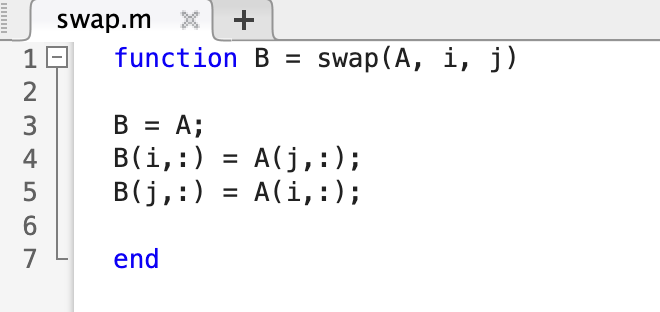
\includegraphics[scale=0.6]{swap.png}}
        \qquad\qquad$swap.m$\label{fig:1}
    \end{minipage}    
    \qquad\qquad\quad
    \begin{minipage}{.4\textwidth}
        \centering
        {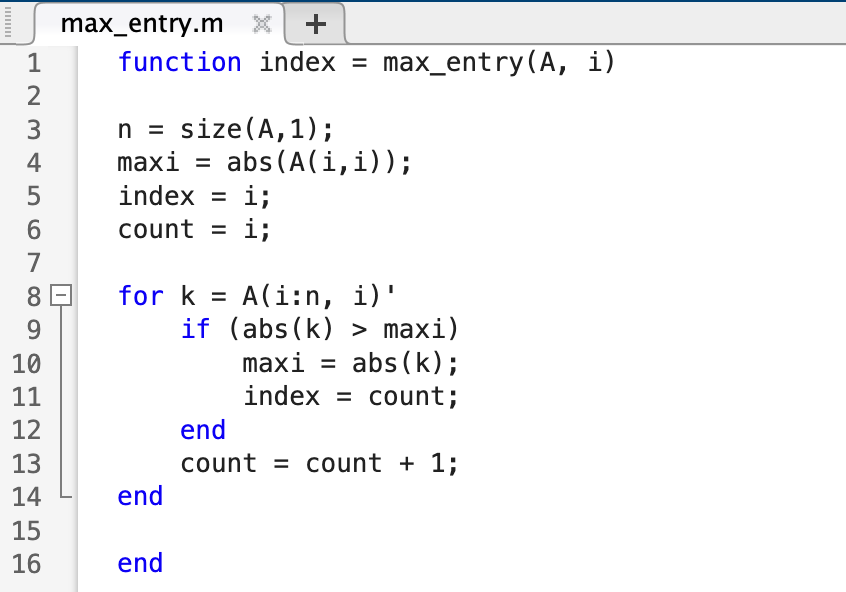
\includegraphics[scale=0.45]{max_entry.png}}
        \qquad\qquad$max\_entry.m$\label{fig:2}
    \end{minipage}        
\end{figure} 

\end{document}